\subsection{Brainstorm}
One of the main techniques applied in the ideation process was brainstorming. In order to get the best outcome from this technique it is important that any idea, no matter the absurdity, is allowed on the drawing. Others may benefit from these seemingly absurd ideas. Early on in the ideation process there was a strong consensus in the group that we find our problem in the waste recycling domain. Figure \ref{fig:wasteTypesBrainstorm} shows the first brainstorm the group made.

\begin{figure}[!ht]
	\centering
	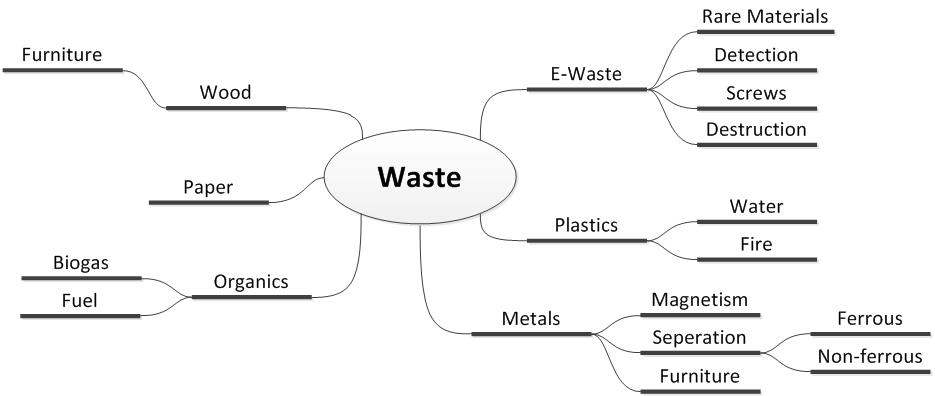
\includegraphics[scale=.5]{./graphics/wasteTypesBrainstorm.jpg}
	\caption{Brainstorm on different areas of waste recycling and possible ways of sorting}
	\label{fig:wasteTypesBrainstorm}
\end{figure}

As can be seen, the two fields of metals and E-waste received the most interest. A vote was held to decide which of the two fields we were going to continue our research on. E-waste was chosen. To further specify the problem of our project another brainstorm was started, this time on different problems within the field of E-waste. The result can be seen in figure \ref{fig:EWasteBrainstorm}.

\begin{figure}[!ht]
	\centering
	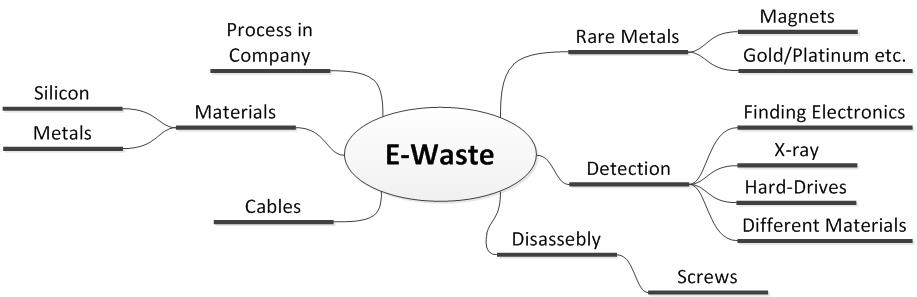
\includegraphics[scale=.5]{./graphics/EWasteBrainstorm.jpg}
	\caption{Brainstorm on problems within the field of E-Waste}
	\label{fig:EWasteBrainstorm}
\end{figure}

No real result came from the brainstorm on E-Waste, and we came to the realisation that more research was needed for us to finalize our project idea. A list of questions was devised and each member was assigned to do research on some of these questions. \\~~\\
At this point we were advised by the supervisors to either make a choice based on the research we had already done, or to go in another direction entirely. It was decided to do a brainstorm entirely focused on concepts, this can be seen in figure \ref{fig:conceptsBrainstorm}.

\begin{figure}[!ht]
	\centering
	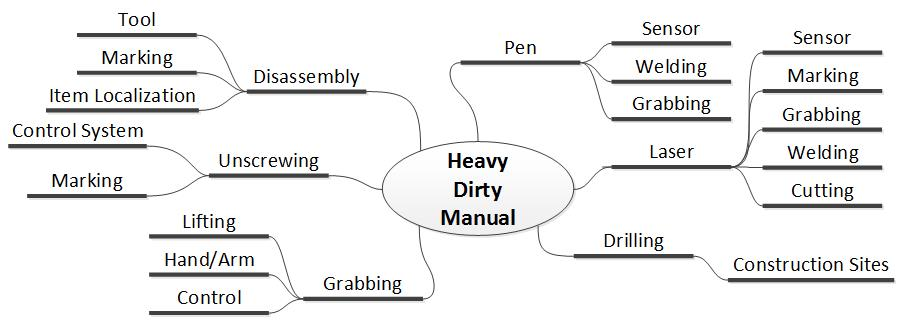
\includegraphics[scale=.5]{./graphics/conceptsBrainstorm.jpg}
	\caption{Brainstorm on possible concepts}
	\label{fig:conceptsBrainstorm}
\end{figure}

Upon finishing the brainstorm the team split into two groups, each group discussing applications for each concept. Ultimately, we decided to focus our project on the development of a flexible welding robot, using a derivation of the pen principle.

\subsection{Conclusion on Innovation}
A lot of time was spent in the beginning trying to find a specific problem to work with, due to the limitation of ideas, no solutions were to be found within the domain of our problem. When reflecting on this process it could have been solved by the following: \\
- Having a team member with Plant as main role. \\
- Having a wider project topic. \\
- Spending all energy of phase one on finding a problem and an idea for a solution. \\
- Using other activities for idea generation, like the six thinking hats. \\
Brainstorms are good for gaining an overview of the members knowledge areas and thoughts. But they are not always brilliant when it comes to generation certain solutions for problems. 